% Data flow diagram
% Author: David Fokkema
\documentclass{standalone}
\usepackage{tikz}
\usetikzlibrary{arrows,quotes,shapes.multipart,arrows.meta}

% Defines a `datastore' shape for use in DFDs.  This inherits from a
% rectangle and only draws two horizontal lines.
\makeatletter
\pgfdeclareshape{datastore}{
  \inheritsavedanchors[from=rectangle]
  \inheritanchorborder[from=rectangle]
  \inheritanchor[from=rectangle]{center}
  \inheritanchor[from=rectangle]{base}
  \inheritanchor[from=rectangle]{north}
  \inheritanchor[from=rectangle]{north east}
  \inheritanchor[from=rectangle]{east}
  \inheritanchor[from=rectangle]{south east}
  \inheritanchor[from=rectangle]{south}
  \inheritanchor[from=rectangle]{south west}
  \inheritanchor[from=rectangle]{west}
  \inheritanchor[from=rectangle]{north west}
  \backgroundpath{
    %  store lower right in xa/ya and upper right in xb/yb
    \pgfset{outer xsep=1.5cm}
    \pgfset{outer ysep=1.5cm}
    \southwest \pgf@xa=\pgf@x \pgf@ya=\pgf@y
    \northeast \pgf@xb=\pgf@x \pgf@yb=\pgf@y
    \pgfpathmoveto{\pgfpoint{\pgf@xa}{\pgf@ya}}
    \pgfpathlineto{\pgfpoint{\pgf@xb}{\pgf@ya}}
    \pgfpathmoveto{\pgfpoint{\pgf@xa}{\pgf@yb}}
    \pgfpathlineto{\pgfpoint{\pgf@xb}{\pgf@yb}}
 }
}
\makeatother

\begin{document}
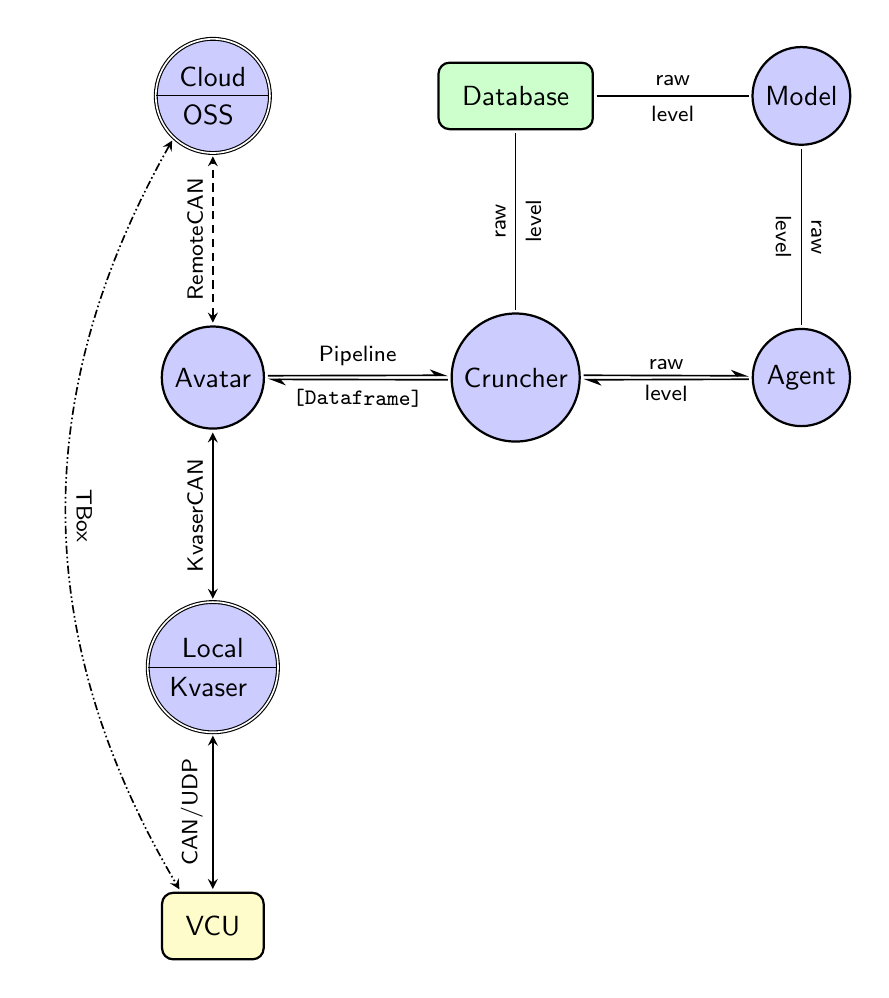
\begin{tikzpicture}[
  font=\sffamily,
  every matrix/.style={ampersand replacement=\&,column sep=2cm,row sep=2cm},
  source/.style={draw,thick,rounded corners,fill=yellow!20,inner sep=.3cm},
  process/.style={draw,thick,circle,fill=blue!20},
  multimodal/.style={circle split,draw,double,fill=blue!20},
  sink/.style={source,fill=green!20},
  datastore/.style={draw,very thick,shape=datastore,inner sep=.3cm},
  dots/.style={gray,scale=2},
  to/.style={->,>=stealth',shorten >=1pt,semithick,font=\sffamily\footnotesize},
  every edge/.style={draw,>=stealth,shorten <=1pt, shorten >=1pt,semithick,font=\sffamily\footnotesize},
  every edge quotes/.style={auto=left,sloped,font=\sffamily\footnotesize},
  every node/.style={align=center}
]
  %every edge/.style={->,>=stealth',shorten >=1pt,semithick,font=\sffamily\footnotesize},


  % Position the nodes using a matrix layout
  \matrix{
    \node[multimodal] (cl) {
      Cloud
      \nodepart{lower}
      OSS
    };
    \& \node[sink] (db) {Database};
    \& \node[process] (mo) {Model}; \\
    \node[process] (av) {Avatar};
    \& \node[process] (cr) {Cruncher};
    \& \node[process] (ag) {Agent}; \\
    \node[multimodal] (kv) {
      Local
      \nodepart{lower}
      Kvaser
    };
    \&
    \& \\
    \node[source] (v) {VCU}; \&  \&\\
  };

  % Draw the arrows between the nodes and label them.
  \draw (db) edge ["raw" above, "level"'] (mo)
        (mo) edge ["raw" above, "level"'] (ag);
  \draw (av.2) edge [arrows={-Stealth[harpoon]},"Pipeline"] (cr.178)
        (cr.2) edge [arrows={-Stealth[harpoon]},"level"'] (ag.178);
  \draw (ag.182) edge [arrows={-Stealth[harpoon]},"raw"] (cr.358)
        (cr.182) edge [arrows={-Stealth[harpoon]},"\texttt{\string[Dataframe\string]}"'] (av.358);
  \draw (cr) edge ["raw", "level"'] (db);
  \draw (kv) edge [<->,"KvaserCAN"] (av);
  \draw (av) edge [<->,densely dashed,"RemoteCAN"] (cl);
  \draw (v) edge [<->,"CAN/UDP"] (kv);
  \draw (cl.227) edge [<->, densely dash dot dot,bend right,"TBox"] (v.133);
\end{tikzpicture}
\end{document}
